% !TEX program = xelatex
\documentclass{beamer}
\usefonttheme[onlymath]{serif}
\setbeamerfont{footnote}{size=\tiny}

% use multiple languages
%% ---- allow CJK usage ---- %%
\usepackage[CJKspace]{xeCJK} % this should be called before Polyglossia
\setCJKmainfont{Noto Serif CJK TC}
\setCJKsansfont{Noto Sans CJK TC}
\setCJKmonofont{Noto Sans Mono CJK TC}
% \setCJKmainfont{Noto Serif JP}
% \setCJKsansfont{Noto Sans JP}
% \setCJKmonofont{Noto Sans Mono CJK JP}

%% ---- ตั้งค่าให้ตัดคำภาษาไทย ---- %%
\XeTeXlinebreaklocale "th"
\XeTeXlinebreakskip = 0pt plus 0pt % เพิ่มความกว้างเว้นวรรคให้ความยาวแต่ละบรรทัดเท่ากัน

%% ---- font settings ---- %%
\usepackage{fontspec}
\defaultfontfeatures{Mapping=tex-text} % map LaTeX formating, e.g., ``'', to match the current font
% To change the main font, uncomment one of the below command.
% \setmainfont{TeX Gyre Termes} % Free Times
% \setsansfont{TeX Gyre Heros} % Free Helvetica
% \setmonofont{TeX Gyre Cursor} % Free Courier
\newfontfamily{\thaifont}[Scale=MatchUppercase,Mapping=textext]{Laksaman} % ตั้งฟอนต์หลักภาษาไทย
\newenvironment{thailang}{\thaifont}{} % create environment for Thai language
\usepackage[Latin,Thai]{ucharclasses} % ตั้งค่าให้ใช้ "thailang" environment เฉพาะ string ที่เป็น Unicode ภาษาไทย
\setTransitionTo{Thai}{\begin{thailang}}
\setTransitionFrom{Thai}{\end{thailang}}

%% ---- spacing between lines ---- %%
\usepackage{setspace}
% \singlespacing % default setting
% \onehalfspacing % recommend using this for Thai language

%% ---- using alphabatic language ---- %%
\usepackage{polyglossia}
\setdefaultlanguage{english} % it is preferrable to set English as the main language, since the numeric system is compatible with most LaTeX features such as 'enumerate' and so on
\setotherlanguages{thai}

\AtBeginDocument\captionsthai % allow captions to be in Thai


%% ---- Title page details ---- %%
\title[Rat nephron]{Rat nephron model review}
\author[C. Sint]{Chanoknun Sintavanuruk 
% \\ (ชนกนันท์ สินธวานุรักษ์; 馬予棟) \inst{1} 
% \and author2 \inst{2}
}
% \institute[shortinst]{\inst{1} affiliation 
% % \and \inst{2} affiliation for author2
% }
\date{\today}

% preambles for Beamer

%% ---- math packages ---- %%
\usepackage{amsmath}
\usepackage{amssymb}
\usepackage{bm} % same functionality as \mathbf{} but for greek letters
\numberwithin{equation}{section} % equation numbers are formatted as <#Section>.<#eq in the section>
\usepackage{cancel}
\renewcommand\CancelColor{\color{red}}

%% ---- define math environment ---- %%
\usepackage{amsthm}

%% ---- hyperref settings ---- %%
% \usepackage{hyperref} % Beamer already has hyperref by default
\usepackage{url}
\usepackage{cite}
\usepackage{natbib}
\usepackage{bibentry}
\usepackage{xcolor}
\hypersetup{
    colorlinks,
    linkcolor={red!50!black},
    citecolor={blue!50!black},
    urlcolor={blue!80!black}
    }

%% ---- misc. ---- %%
\usepackage{mhchem} % use chemistry notation
\newcommand\scalemath[2]{\scalebox{#1}{\mbox{\ensuremath{\displaystyle #2}}}} % scale display math environment
\usepackage{lipsum}
\usepackage{metalogo} % for extended LaTeX logo such as XeTeX
\usepackage{subcaption} % allowing subfigure environment
% \usepackage[section]{placeins} % ensure floats do not go into the next section and allow the use of \FloatBarrier
\usepackage{graphicx} % allow cropping and rotating images

%% ---- Theme choice ---- %%
\usetheme{metropolis}
% \usetheme{Berkeley}
% \usecolortheme{beaver}
% \usecolortheme{dove}
% \usecolortheme{spruce}
% \logo{\large \XeTeX{}}

%% ---- show TOC after sections ---- %%
% \AtBeginSection[]
% {
%     \begin{frame}
%         \frametitle{Outline}
%         \tableofcontents[currentsection]
%     \end{frame}
%     }

%% ---- Show notes ---- %%
\usepackage{pgfpages}
% \setbeameroption{show notes}
% \setbeameroption{show notes on second screen=right}
% for working around text color bug when using XeLaTeX
\makeatletter 
\def\beamer@framenotesbegin{% at beginning of slide
     \usebeamercolor[fg]{normal text}
      \gdef\beamer@noteitems{}% 
      \gdef\beamer@notes{}% 
}
\makeatother

%% ---- page numbers ---- %%
% \setbeamertemplate{page number in head/foot}[totalframenumber]\setbeamertemplate{navigation symbols}{\footnotesize\usebeamertemplate{page number in head/foot}}

%% ---- figure numbering ---- %%
\setbeamertemplate{caption}[numbered]

\setbeamerfont{caption}{size=\scriptsize}

\begin{document}
% Title page frame
\begin{frame}
    \titlepage 
\end{frame}
% Remove logo from the next slides
\logo{}

% Outline frame
\begin{frame}{Outline}
    \tableofcontents
\end{frame}

\section{Overview of structures}
\begin{frame}{Compartments}
    \nobibliography*
    \begin{enumerate}
        \item nephrons
        \item medullary vasculature
        \item medullary interstitium
    \end{enumerate}
    \begin{figure}
        \centering
        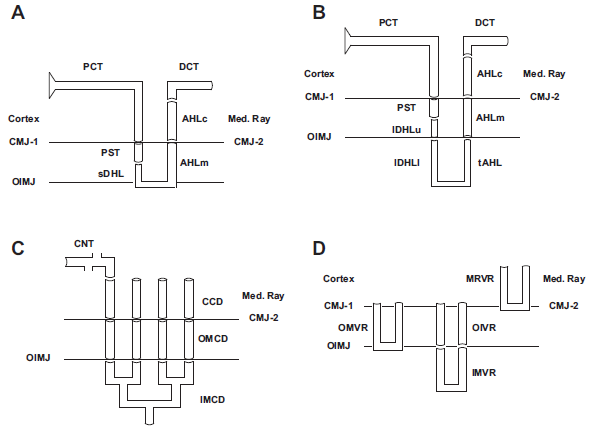
\includegraphics[width=0.5\textwidth]{figures/compartments.png}
        \caption{model compartments \citep{Weinstein2017}\footnote[frame,1]{\tiny\bibentry{Weinstein2017}}}
    \end{figure}
    \note{
        The model has 3 compartments: nephrons, medullary vasculature and medullary interstitium.
        \\~\\
        Nephrons and blood vessels are divided into multiple segments.
        In terms of spatial dimension, each segment has only length with the direction either going up or down the medulla.
        \\~\\
        The interstitial compartment is divided into 8 different homogeneous sub-compartments; each represents different depth and contains some segments of blood vessels and nephrons.
    }

\end{frame}

\begin{frame}{Tubular segments of nephrons (1/2)}
    \note<1>{
        The nephron compartment is composed of many distinct tubular segments which can be grouped into unbranched segments and the distal nephron ensembles or the collecting ducts.
    }
    \begin{columns}
        %% ---- left column ---- %%
        \begin{column}{0.5\linewidth}
            \begin{enumerate}
                \item unbranched segments
                \begin{enumerate}
                    \item Superficial (SF) nephrons
                    \item Juxtamedullary (JM) nephrons
                \end{enumerate}
                \item \textcolor<2->{lightgray}{distal nephron ensembles: collecting ducts}
            \end{enumerate}
        \end{column}\hfill
        %% ---- right column ---- %%
        \begin{column}{0.5\linewidth}
            \onslide<2->{\begin{figure}
                \centering
                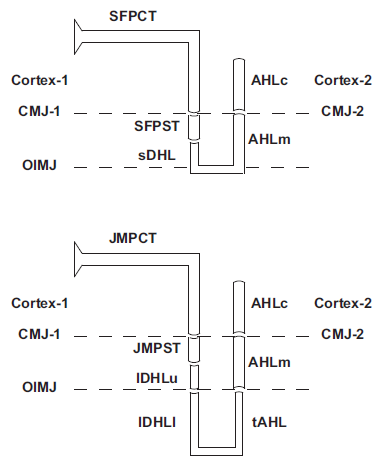
\includegraphics[width=.82\textwidth]{figures/unbranched.png}
                \caption{Unbranched tubules \citep{Weinstein2015}\footnote<2->[frame,1]{\tiny{\bibentry{Weinstein2015}}}}
            \end{figure}}
        \end{column}
    \end{columns}    
    \note<2>{
        The unbranched segments are connected in series in mainly two different ways resulting the superficial or SF and juxtamedullary or JM nephron.
        \\~\\
        These nephrons have distal segments that are identical, which are the thick ascending limbs, or AHL, in the outer medulla and the cortex. 
        Meanwhile, the proximal convoluted tubule, or PCT, and straight tubule, or PST, of these two differ in the glomerular filtration rate, which determines the initial flow and pressure at the PCT, and ion permeabilities --- which are mostly higher in the JM nephron.
        \\~\\
        For the segments in the middle, the SF nephron has only one segment of the descending Henle's limb, or DHL, at the outer medulla; while in JM nephron, DHL descends into the inner medulla in 5 different depths and comes back up via thin ascending Henle's limb, or tAHL.
    }
\end{frame}

\begin{frame}{Tubular structure of DHL and tAHL}
    \begin{figure}
        \centering
        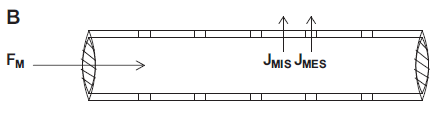
\includegraphics[width=0.5\textwidth]{figures/thin_tubule.png}
        \caption{transepithelial fluxes of DHL and tAHL \citep{Weinstein2015}\footnote[frame,1]{\tiny{\bibentry{Weinstein2015}}}}
    \end{figure}
    \begin{figure}
        \centering
        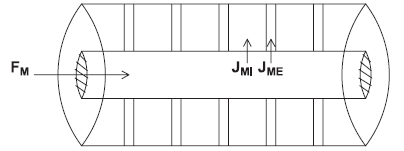
\includegraphics[width=0.45\textwidth]{figures/thick_tubule.png}
        \caption{epithelial cells and lateral interspaces \citep{Weinstein2010}\footnote[frame,2]{\tiny{\bibentry{Weinstein2010}}}}
    \end{figure}
    \note{
        These segments of DHL and tAHL in the middle, which are parts of the thin Henle's loop, do not have cellular structures and lateral interspaces.
        So transepithelial fluxes of ions and water are all passive.
        \\~\\
        The rest of the tubular segments including those of collecting ducts, however, have epithelial cells and lateral interspaces included which separate the luminal and the basement membranes.
    }
\end{frame}

\begin{frame}{Tubular segments of nephrons (2/2)}
    \note{
        In distal nephron, the distal convoluted tubules, or DCT, come after the AHL.
        So there are total of 6 different profiles of DCT which receive flow from either 1 SF nephron or 5 JM nephrons.
        All of these flows into the connecting tubule, or CNT, in the way that each CNT are identical.
        \\~\\
        Similar branching can also be found at the inner medullary collecting ducts, or IMCD.
    }
    \begin{columns}
        %% ---- left column ---- %%
        \begin{column}{0.5\linewidth}
            \begin{enumerate}
                \item \textcolor{lightgray}{unbranched segments}
                \begin{enumerate}
                    \item \textcolor{lightgray}{Superficial (SF) nephrons}
                    \item \textcolor{lightgray}{Juxtamedullary (JM) nephrons}
                \end{enumerate}
                \item distal nephron ensembles: collecting ducts
            \end{enumerate}
        \end{column}\hfill
        %% ---- right column ---- %%
        \begin{column}{0.5\linewidth}
            \onslide{\begin{figure}
                \centering
                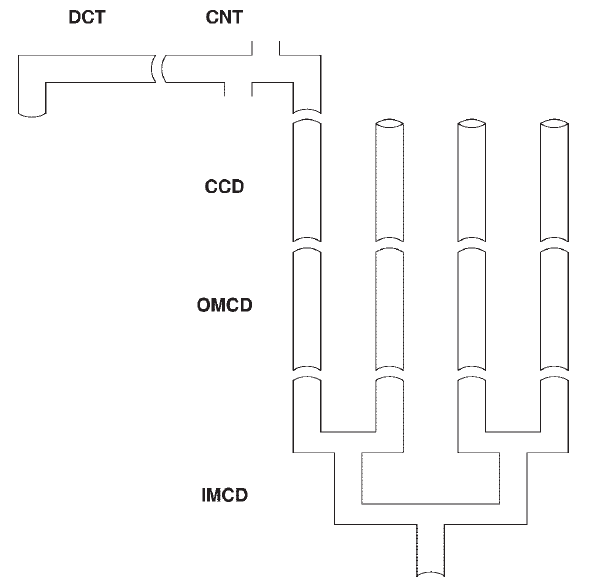
\includegraphics[width=.90\textwidth]{figures/distal_nephron.png}
                \caption{distal nephron \citep{Weinstein2008}\footnote[frame,1]{\tiny{\bibentry{Weinstein2008}}}}
            \end{figure}}
        \end{column}
    \end{columns}    
\end{frame}

\begin{frame}{Vasa recta}
    \onslide<2>{AVR:DVR $= 2:1$.}
    \begin{figure}
        \centering
        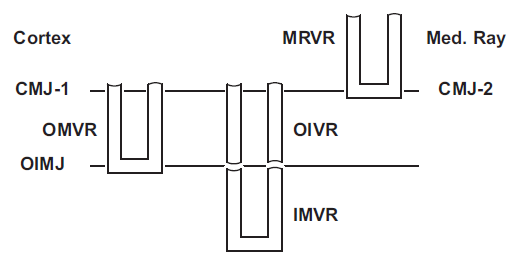
\includegraphics[width=0.6\textwidth]{figures/vasa_recta.png}
        \caption{7 distinct types of vasa recta \citep{Weinstein2017}\footnote[frame,1]{\tiny\bibentry{Weinstein2017}}}
    \end{figure}
    \note<1>{
        In the vascular compartments, there are 5 different kinds of vasa recta: the short one, the long ones which reaches 5 different depths, and the medullary ray vasa recta, or MRVR, which is the blood vessels that surround the cortical AHL.
        \\~\\
        Similar to the thin Henle's loop, vasa recta are assumed to not have cellular and paracellular structures.
        Each types of vasa recta is composed of segments with 3 different profiles of solute permeability, first at outer medulla and MRVR, which is assumed to be the same as MRVR, second at the inner medulla vasa recta, or IMVR, at the descending direction; and this is different from the third profile of ascending IMVR.
    }
    \note<2>{
        It is also worth noting that, the branching of vasa recta is represented by the ratio between the number ascending vasa recta or AVR to the descending DVR; which was set to be $2:1$.
    }
\end{frame}

\begin{frame}{Medullary interstitium}
    8 sub-compartments
    \begin{figure}
        \centering
        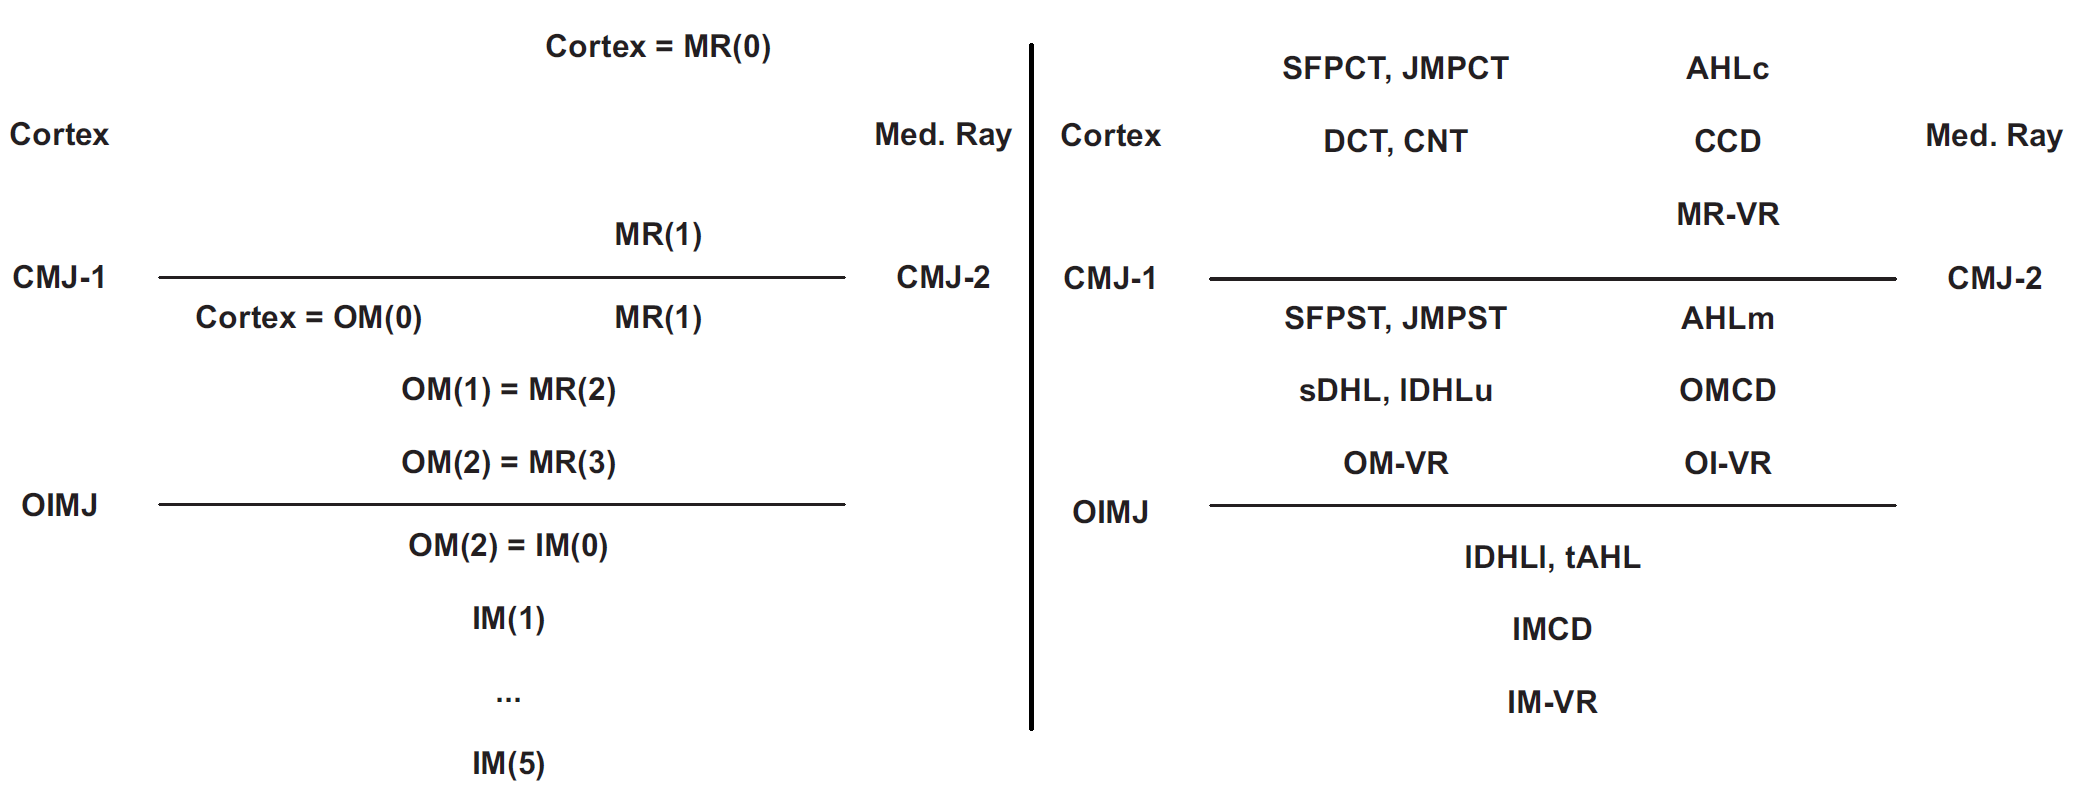
\includegraphics[width=0.95\textwidth]{figures/interstitium.png}
        \caption{interstitial sub-compartments \citep{Weinstein2017}\footnote[frame,1]{\tiny\bibentry{Weinstein2017}}}
    \end{figure}
    \note<1>{
        The third and last compartment is the medullary interstitium which is divided into 8 sub-compartments: 2 outer medulla, 5 inner medullae, and part of medullary ray that reaches the superficial layer.
        The cortical interstitium is not included and its solute concentrations and hydrostatic pressure are kept constant.
        \\~\\
        At the cortex, we have the PCT of SF and JM nephron, DCT, and CNT.
        \\~\\
        At the outer medulla junction, the cortex-medulla junction is separated into the part that continues from the cortex, which contains the PST, and from the medullary ray, which has the distal portion of medulla AHL.
        The two outer medulla sub-compartments then contain the short DHL, upper long DHL, and the outer medullary collecting duct and vasa recta.
    }
    \note<2>{
        The inner medulla has 5 levels of depth after the outer-inner medullary junction.
        These contain the rest of the thin Henle's loop, and the inner medullary collecting ducts and vasa recta.
        \\~\\
        Lastly, the medullary ray.
        This contains the AHL, cortical collecting ducts, or CCD, and the MRVR.
    }
\end{frame}

\section{Model formulation}

\begin{frame}{Thick tubules (with cellular structures)}
    \begin{columns}
        \begin{column}{0.45\linewidth}
            \begin{enumerate}
                \item lumen (M)
                \item epithelial cell (I)
                \item lateral interspace (E)
            \end{enumerate}
        \end{column}

        \begin{column}{0.55\linewidth}
            \begin{figure}
                \centering
                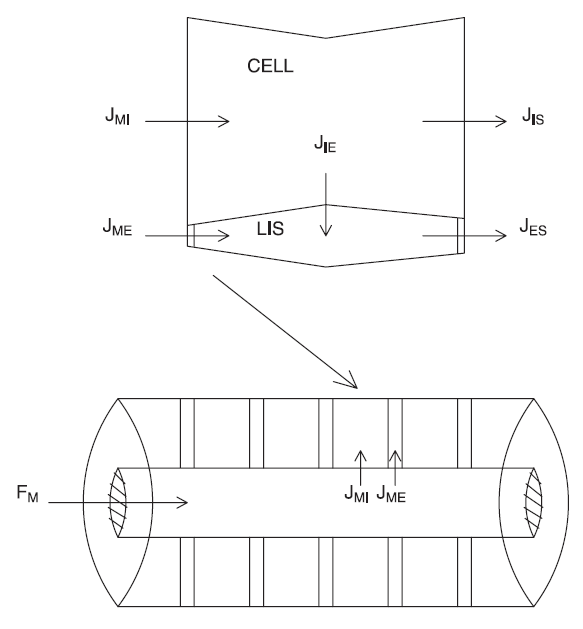
\includegraphics[width=.75\textwidth]{figures/epithelium.png}
                \caption{epithelial cells and LIS \citep{Weinstein1998}\footnote[frame,1]{\tiny\bibentry{Weinstein1998}}}
            \end{figure}
        \end{column}
    \end{columns}
\end{frame}

\begin{frame}{Thick tubules: lumen (M)}
    \onslide<1->{balance equations:
    \begin{align}
        \frac{\partial A_\mathrm{M}}{\partial t} &= -\frac{\partial F_\mathrm{vM}}{\partial x}-B_\mathrm{M}\left(J_\mathrm{vME}+J_\mathrm{vMI}\right),\\
        \frac{\partial }{\partial t}\left(A_\mathrm{M}C_{\mathrm{M},i}\right) &= -\frac{\partial F_{\mathrm{M},i}}{\partial x}-B_\mathrm{M}\left(J_{\mathrm{ME},i}+J_{\mathrm{ME},i}\right)+s_{\mathrm{M},i}.
    \end{align}}
    \begin{figure}
        \centering
        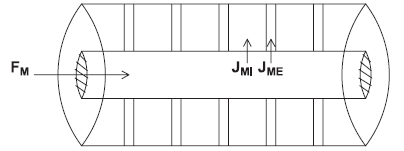
\includegraphics[width=0.7\textwidth]{figures/thick_tubule.png}
    \end{figure}
\end{frame}

\begin{frame}{Thick tubules: cells (I) \& LIS (E)}
    balance equations for $\alpha$ ($\alpha$ represents I or E.):
    \begin{align}
        \frac{\partial V_{\alpha}}{\partial t} &= J_{\mathrm{vM}\alpha} \mp J_{\mathrm{vIE}}-J_{\mathrm{v}\alpha\mathrm{S}},\\
        \frac{\partial}{\partial t}\left(V_{\alpha}C_{\alpha,i}\right) &= J_{\mathrm{M}\alpha,i} \mp J_{\mathrm{IE},i}-J_{\alpha\mathrm{S},i}+s_{\alpha,i}
    \end{align}
    \begin{figure}
        \centering
        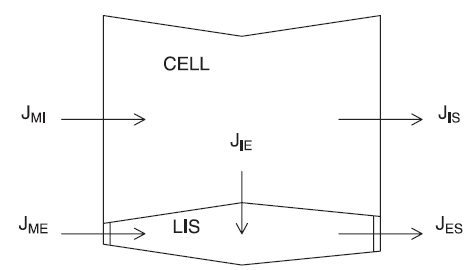
\includegraphics[width=0.5\textwidth]{figures/cell_LIS.png}
    \end{figure}
\end{frame}

\begin{frame}{Thin tubules}
    Only lumen:
    \begin{align}
        \frac{\partial A_\mathrm{M}}{\partial t} &= -\frac{\partial F_\mathrm{vM}}{\partial x}-B_\mathrm{M}\left(J_\mathrm{vMS}+J_\mathrm{vMS}\right),\\
        \frac{\partial }{\partial t}\left(A_\mathrm{M}C_{\mathrm{M},i}\right) &= -\frac{\partial F_{\mathrm{M},i}}{\partial x}-B_\mathrm{M}\left(J_{\mathrm{MS},i}+J_{\mathrm{MS},i}\right)+s_{\mathrm{M},i}.
    \end{align}
    \begin{figure}
        \centering
        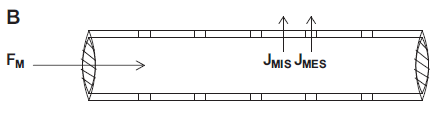
\includegraphics[width=0.75\textwidth]{figures/thin_tubule.png}    
        \caption{luminal flow \& transepithelial fluxes \citep{Weinstein2015}\footnote[frame,1]{\tiny{\bibentry{Weinstein2015}}}}
    \end{figure}
\end{frame}

\begin{frame}{Blood vessels (C)}
    \onslide<1->{
        Only lumen \citep{Weinstein2017}\footnote[frame,1]{\tiny{\bibentry{Weinstein2017}}}:
        \begin{align}
            \frac{\partial F_\mathrm{vC}}{\partial x} &= - B_{\mathrm{C}} J_\mathrm{vCS},\\
            \frac{\partial F_{\mathrm{C},i}}{\partial x} &= -B_\mathrm{C}J_{\mathrm{CS},i}+s_{\mathrm{C},i}.
        \end{align}
        }
    \onslide<2->{
        Relation between blood ($F_{\mathrm{bC}}$) and volume flow ($F_\mathrm{vC}$):
        \begin{align}
            F_\mathrm{vC}&=F_\mathrm{bC}\left(1-\mathrm{Hct}\right),\\
            0 &= \frac{\partial}{\partial x}\left(F_\mathrm{bC}\cdot\mathrm{Hct}\right).
        \end{align}
            }
\end{frame}

\begin{frame}{Solute ($J_{\alpha\beta,i}$) and water fluxes ($J_{\mathrm{v}\alpha\beta}$)}
    % *$\alpha,\beta$ represents different compartments . 
    Water fluxes \citep{Weinstein1983}\footnote[frame,1]{\tiny{\bibentry{Weinstein1983}}}:
    \begin{multline}
        J_{\mathrm{v}\alpha\beta} = 
            L_{\mathrm{v}\alpha\beta}A_{\alpha\beta}\bigg(P_\alpha-P_\beta+\pi_\beta-\pi_\alpha\\
            +RT\sum_i\sigma_{\alpha\beta,i}\left(C_{\beta,i}-C_{\alpha,i}\right)\bigg)
    \end{multline}
    Solute fluxes:
    \begin{multline}
        J_{\alpha\beta,i} = (1-\sigma_{\alpha\beta,i})J_{\mathrm{v}\alpha\beta}\overline{C}_{\alpha\beta,i}\\
        +z_ih_{\alpha\beta,i}A_{\alpha\beta}\phi_{\alpha\beta}\left(\frac{C_{\alpha,i}-C_{\beta,i}e^{-z_i\phi_{\alpha\beta}}}{1-e^{-z_i\phi_{\alpha\beta}}}\right)\\
        +A_{\alpha\beta}\sum_j L_{\alpha\beta;i,j}\mu_{\alpha\beta,j} + J^{\mathrm{act}}_{\alpha\beta,i}
    \end{multline}

\end{frame}
        
\begin{frame}{Hydrostatic pressure (M \& C)}
    Poiseuille's flow equations:
    \begin{itemize}
        \item tubules \citep{Weinstein1998}\footnote[frame,1]{\tiny{\bibentry{Weinstein1998}}}:
        \begin{equation}
            \frac{\partial P_\mathrm{M}}{\partial x}+\frac{8\pi\eta}{A^2_\mathrm{M}}\cdot F_\mathrm{vM}=0,
        \end{equation}
        \item vessels \citep{Weinstein2017}\footnote[frame,2]{\tiny{\bibentry{Weinstein2017}}}:
        \begin{equation}
            \frac{\partial P_\mathrm{C}}{\partial x}+\frac{8\pi\eta_\mathrm{C}}{A^2_\mathrm{C}}\cdot F_\mathrm{bC}=0.
        \end{equation}
    \end{itemize}
\end{frame}

\begin{frame}{Tubular compliance}
    Thick tubules of nephron are compliant \citep{Weinstein2007,Weinstein2015}\footnote[frame,1]{\tiny{\bibentry{Weinstein2007}\\ \bibentry{Weinstein2015}}}:
    \begin{align}
        R_\mathrm{M}&=R_{\mathrm{M}0}\left(1+\frac{1}{2}\tanh\big(\nu_\mathrm{M}(P_\mathrm{M}-P_\mathrm{S})\big)\right)
    \end{align}
    Compliant lateral interspaces:
    \begin{align}
        A_\mathrm{ES} &=A_{\mathrm{ES}0}\left(1+\nu_\mathrm{AE}(P_\mathrm{M}-P_\mathrm{S})\right),\\
        V_\mathrm{E} &=V_{\mathrm{E}0}\left(1+\nu_\mathrm{VE}(P_\mathrm{M}-P_\mathrm{S}).\right)
    \end{align}
\end{frame}

\begin{frame}{Flow-dependent transport of PCT}
    PCT transporter density parameters ($\mathrm{Par}$) depend on torque of microvilous ($T_M$)\citep{Weinstein2007}\footnote[frame,1]{\tiny{\bibentry{Weinstein2007}}}:
    \begin{align}
        \mathrm{Par} &= \mathrm{Par}_0\left(1+T_\mathrm{s}\left(\frac{T_\mathrm{M}}{T_{\mathrm{M}0}}\right)\right)\\
        T_\mathrm{M} &= \frac{8\eta l F_{\mathrm{vM}}}{R_\mathrm{M}^2}\left(1+\frac{l+\delta}{R_\mathrm{M}}+\frac{l^2}{2R^2_\mathrm{M}}\right)
    \end{align}
    \begin{figure}
        \centering
        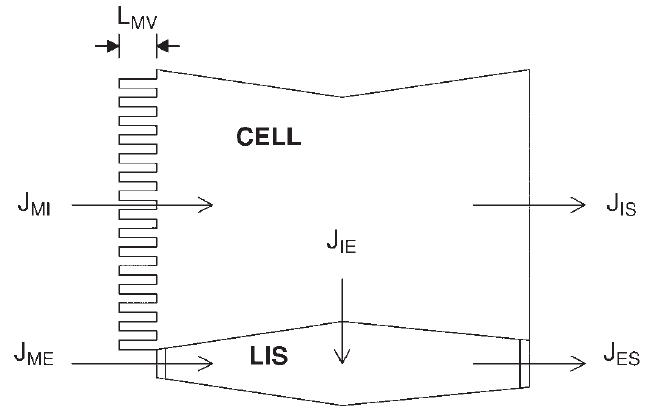
\includegraphics[width=0.4\textwidth]{figures/PCT_epithelium.png}
    \end{figure}
\end{frame}

\begin{frame}{Solute generation ($s_{\mathrm{\alpha},i}$) in M \& C}
    \onslide<1->{Acid-base (\ce{ H+ + B <=> HB }) \citep{Weinstein2017}\footnote[frame,1]{\tiny\bibentry{Weinstein2017}}:
    \begin{gather}
        s_{\alpha,\mathrm{B}}+s_{\alpha,\mathrm{HB}}=0\\
        C_{\mathrm{M},\ce{ H+ }} = K_1\frac{C_{\mathrm{M},\ce{ HB }_1}}{C_{\mathrm{M},\ce{ B- }_1}} = K_2\frac{C_{\mathrm{M},\ce{ HB }_2}}{C_{\mathrm{M},\ce{ B- }_2}} = \ldots\\
        \sum_iz_is_{\mathrm{M},i}=0,\quad \sum_iz_iC_{\mathrm{M},i}=0
    \end{gather}}
    \onslide<2->{\ce{ CO2 }: (\ce{ H+ + HCO3^- <=> H2CO3^- <=>[$k_+$][$k_-$] H2O + CO2}):
    \begin{gather}
        s_{\alpha,\ce{ HCO3 }} + s_{\alpha,\ce{ H2CO3 }} + s_{\alpha,\ce{ CO2 }} = 0\\
        s_{\mathrm{I},\ce{ HCO3 }} + s_{\mathrm{I},\ce{ H2CO3 }} + s_{\mathrm{I},\ce{ CO2 }} = M_{\mathrm{I},\ce{ CO2 }}
    \end{gather}}
\end{frame}    

\begin{frame}{Hemoglobin buffering species}
    
\end{frame}

\begin{frame}{Global variables}
    
\end{frame}

\begin{frame}{Tubulo-glomerular feedback (TGF)}
    
\end{frame}

\begin{frame}{End-DCT pressure}
    
\end{frame}

\begin{frame}{Interstitial variables}
    
\end{frame}

\begin{frame}[allowframebreaks]{References}
    \bibliographystyle{plainnat}
    \tiny\bibliography{bibliography}
\end{frame}

\end{document}